%%%%%%%%%%%%%%%%%%%%%%%%%%%%%%%%%%%%%%%%%
% Beamer Presentation
% LaTeX Template
% Version 1.0 (10/11/12)
%
% This template has been downloaded from:
% http://www.LaTeXTemplates.com
%
% License:
% CC BY-NC-SA 3.0 (http://creativecommons.org/licenses/by-nc-sa/3.0/)
%
%%%%%%%%%%%%%%%%%%%%%%%%%%%%%%%%%%%%%%%%%

%----------------------------------------------------------------------------------------
%	PACKAGES AND THEMES
%----------------------------------------------------------------------------------------

\documentclass[14pt]{beamer}

\mode<presentation> {

% The Beamer class slide themes
\usetheme{Madrid} %i was using this one

% Beamer class color themes

%\usecolortheme{albatross}

%\setbeamertemplate{footline} % To remove the footer line in all slides uncomment this line
%\setbeamertemplate{footline}[page number] % To replace the footer line in all slides with a simple slide count uncomment this line

%\setbeamertemplate{navigation symbols}{} % To remove the navigation symbols from the bottom of all slides uncomment this line
}

\usepackage{graphicx} % Allows including images
\usepackage{booktabs} % Allows the use of \toprule, \midrule and \bottomrule in tables
\usepackage{hyperref}
\usepackage{helvet}

%----------------------------------------------------------------------------------------
%	TITLE PAGE
%----------------------------------------------------------------------------------------

\title[RNAseq]{Everything you wanted to know about RNAseq} % The short title appears at the bottom of every slide, the full title is only on the title page

\author{C. Ryan Campbell} % Your name
\institute[Duke] % Your institution as it will appear on the bottom of every slide, may be shorthand to save space
{
Duke University \\ % Your institution for the title page
\medskip
\textit{c.ryan.campbell@duke.edu} % Your email address
}
\date{12 Sept 2017} % Date, can be changed to a custom date

\begin{document}

\begin{frame}
\titlepage % Print the title page as the first slide
\end{frame}

\begin{frame}
\frametitle{Overview} % Table of contents slide, comment this block out to remove it
\tableofcontents % Throughout your presentation, if you choose to use \section{} and \subsection{} commands, these will automatically be printed on this slide as an overview of your presentation
\end{frame}

%----------------------------------------------------------------------------------------
%	PRESENTATION SLIDES
%----------------------------------------------------------------------------------------

%------------------------------------------------
\section{RNAseq} 
%------------------------------------------------

\subsection{Goals} 

%------------------------------------------------
\begin{frame}
\frametitle{Today's Goals}
%what students should know/learn today
\begin{itemize}
	\item How does RNAseq work?
	\item What are the benefits?
	\item What are the challenges?
	\item[]
	\item Meet your group!
	%\sffamily
\end{itemize}
\end{frame}


%------------------------------------------------
\subsection{Introduction}
%------------------------------------------------

%------------------------------------------------
\begin{frame}
\frametitle{Dotstorming}
\begin{itemize}
	\item What questions did you have?
	\item \href{https://dotstorming.com/b/59b6a35f3b45421106effc50}{Dotstorming Board}
	\item Write your question
	\item Vote on others
	\item (Take 5 mins)
\end{itemize}
\end{frame}

%------------------------------------------------
\begin{frame}
\frametitle{A Parable}
\begin{columns}
	\begin{column}{0.5\textwidth}
		\begin{itemize}
			\item<+-> Steve and Susan wanted to know how water affects plant growth
			\item<+-> They decide to grow the same vine in 6 different pots by the window in their classroom
		\end{itemize}
		\end{column}
	\begin{column}{0.5\textwidth}
		\begin{center}
     		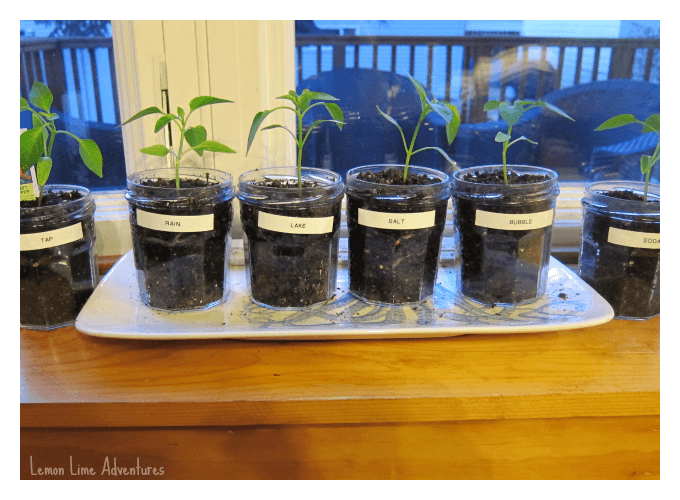
\includegraphics[width=1\textwidth]{images_20170912_vines.png}
     	\end{center}
	\end{column}
\end{columns}
\end{frame}

%------------------------------------------------
\begin{frame}
\frametitle{A Parable}
\begin{columns}
	\begin{column}{0.5\textwidth}
		\begin{itemize}
			\item<+-> Each day they give the pots 2 cups of water
			\item<+-> At the end of 3 months they measure the length of the vine
			\item<+-> What is wrong with this ``experiment''?
		\end{itemize}
		\end{column}
	\begin{column}{0.5\textwidth}
		\begin{center}
     		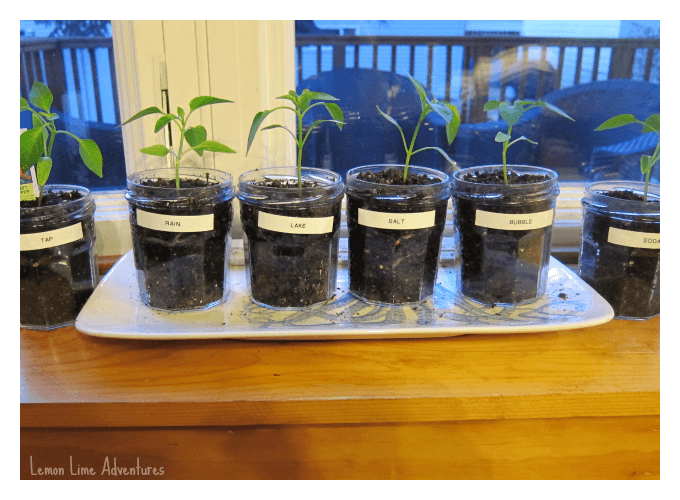
\includegraphics[width=1\textwidth]{images_20170912_vines.png}
     	\end{center}
	\end{column}
\end{columns}
\end{frame}

%------------------------------------------------
\subsection{Central Dogma}
%------------------------------------------------

%------------------------------------------------
\begin{frame}
\frametitle{Central Dogma}
\begin{itemize}
	\item<+-> DNA codes for
	\item<+-> RNA codes for
	\item<+-> Protien
\end{itemize}
\end{frame}

%------------------------------------------------
\begin{frame}
\frametitle{DNA}
	\begin{itemize}
		\item<+-> Static, non-changing
		\item<+-> You're stuck with the genome you have
		\item<+-> Good for investigating large scale and inflexible impacts of environment
		\item<+-> A written record of selection over time
		\begin{itemize}
			\item (or population size changes)
			\item (or species histories) 
		\end{itemize}
	\end{itemize}
\end{frame}

%------------------------------------------------
\begin{frame}
\frametitle{RNA}
	\begin{itemize}
		\item<+-> Dynamic, ever-changing
		\item<+-> Transcribed ``as needed'' from DNA
		\item<+-> Only exons, introns are spliced out
	\end{itemize}
\end{frame}

%------------------------------------------------
\begin{frame}
\frametitle{Protein}
	\begin{itemize}
		\item<+-> Final product of central dogma
		\item<+-> ``Action item'' from the list
		\item<+-> Performs a task within the cell
	\end{itemize}
\end{frame}

%------------------------------------------------
%%UNCOMMENT
\begin{frame}
\frametitle{RNAseq}
	\begin{itemize}
		\item<+-> Sequencing the RNA molecules in a cell
		\begin{itemize}
			\item<+-> Use as a proxy for identifying active proteins
		\end{itemize}
		\item<+-> Why not DNA?
		\begin{itemize}
			\item<+-> Static, doesn't change based on cell function or status
			\item<+-> Doesn't tell us where the genes are (annotation)
		\end{itemize}
		\item<+-> Why not Proteins?
		\begin{itemize}
			\item<+-> Unstable
			\item<+-> Difficult to collect and quantify
		\end{itemize}
	\end{itemize}
\end{frame}

%------------------------------------------------
\subsection{Measuring RNA}
%------------------------------------------------

%------------------------------------------------
\begin{frame}
\frametitle{Measuring RNA}
	\begin{enumerate}
		\item<+-> Generate cDNA
		\item<+-> Prepare a sequencing library
		\item<+-> (Next-Gen) Sequence!!!
	\end{enumerate}
\end{frame}

%------------------------------------------------
\begin{frame}
\frametitle{Generate cDNA}
\begin{columns}
	\begin{column}{0.5\textwidth}
	\footnotesize
	\begin{itemize}
		\item<+-> Isolate RNA from cells and use deoxyribonuclease (DNAse) to remove accidental DNA
		\item<+-> Select for poly-A tails to enrich for mature RNA (often with magnetic beads)
		\item<+-> Reverse transcribe the RNA into cDNA (lasts longer)
		\begin{itemize}
			\footnotesize
			\item<+-> Lose strand info
			\item<+-> Can be kept with labeling
		\end{itemize}
	\end{itemize}
	\end{column}
	\begin{column}{0.5\textwidth}
	\begin{center}
    	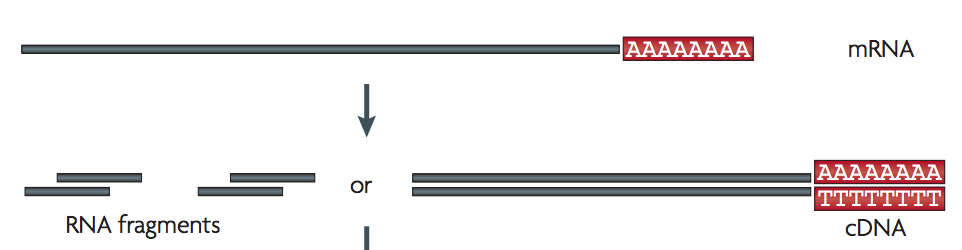
\includegraphics[width=1\textwidth]{images_20170912_cDNA.png}
    \end{center}
	\end{column}
\end{columns}
\end{frame}

%------------------------------------------------
\begin{frame}
\frametitle{prepare a sequencing library}
\begin{columns}
	\begin{column}{0.5\textwidth}
	\begin{itemize}
		\item<+-> Take the now-cDNA into a standard library prep
		\item<+-> Add adapters
		\item<+-> Amplify (with PCR) and sequence
	\end{itemize}
	\end{column}
	\begin{column}{0.5\textwidth}
	\begin{center}
    	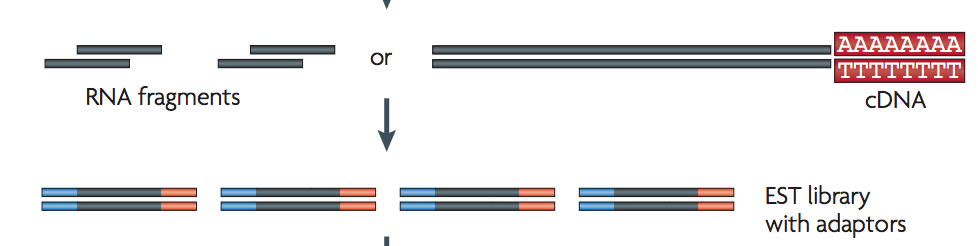
\includegraphics[width=1\textwidth]{images_20170912_libprep.png}
    \end{center}
	\end{column}
\end{columns}
\end{frame}

%------------------------------------------------
\begin{frame}
\frametitle{NGS!!!}
\begin{columns}
	\begin{column}{0.5\textwidth}
	\begin{itemize}
		\item<+-> Single-end or paired-end
		\begin{itemize}
			\item<+-> Because genes are often shorter than the full length of paired-end, data is analyzed one end at a time
		\end{itemize}
		\item<+-> Generate billions of reads
		\item<+-> ``fastq'' format
	\end{itemize}
	\end{column}
	\begin{column}{0.5\textwidth}
	\begin{center}
    	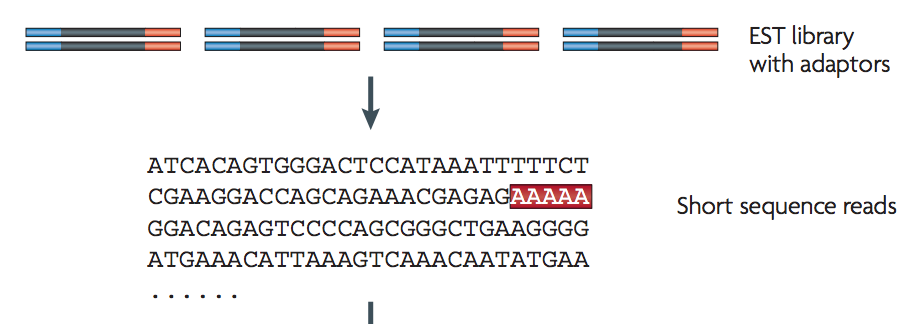
\includegraphics[width=1\textwidth]{images_20170912_seq.png}
    \end{center}
	\end{column}
\end{columns}
\end{frame}

%------------------------------------------------
\begin{frame}
\frametitle{fastq Format}
\begin{columns}
	\begin{column}{0.5\textwidth}
	\begin{enumerate}
		\item<+-> Sequence header - information regarding the machine
		\item<+-> Sequence content - bases
		\item<+-> Sequence header - repeat of above (+ instead of @)
		\item<+-> Sequence quality - ASCII coded
	\end{enumerate}
	\end{column}
	\begin{column}{0.5\textwidth}
	\begin{center}
    	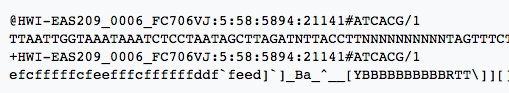
\includegraphics[width=1\textwidth]{images_20170912_fastq.png}
    \end{center}
	\end{column}
\end{columns}
\end{frame}



%------------------------------------------------
\begin{frame}
\frametitle{Now what do we do?}
\begin{columns}
	\begin{column}{0.5\textwidth}
	\begin{itemize}
		\item<+-> Map reads to a genome/annotation
		\begin{itemize}
			\item (or not! - \textit{de novo})
		\end{itemize}
		\item<+-> Count depth of reads at each gene
		\item<+-> Infer amount of RNA (and thus protein) in the cells
	\end{itemize}
	\end{column}
	\begin{column}{0.5\textwidth}
	\begin{center}
    	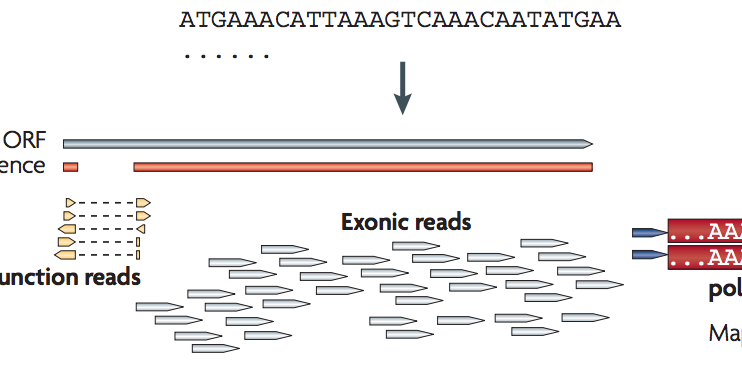
\includegraphics[width=1\textwidth]{images_20170912_map.png}
    \end{center}
	\end{column}
\end{columns}
\end{frame}

%------------------------------------------------
\begin{frame}
\frametitle{Statistics}
	\begin{itemize}
		\item<+-> Map to genes? or exons?
		\begin{itemize}
			\item Exon mapping can help determine splice variants
		\end{itemize}
		\item<+-> Standardize by amount of data
		\begin{itemize}
			\item<+-> FPM - Fragments (mapped) Per Million bases (of NGS data)
		\end{itemize}
		\item<+-> Standardize by length of gene as well
		\begin{itemize}
			\item<+-> FPKM - Fragments Per Kilobase of transcript per Million mapped reads
		\end{itemize}
		\item<+-> Sampling error at low numbers
		\begin{itemize}
			\item<+-> Not always normal variance (can't sample below 0)
			\item<+-> Poisson distribution
		\end{itemize}
	\end{itemize}
\end{frame}

%------------------------------------------------
\begin{frame}
\frametitle{Many choices produce many results}
	\begin{itemize}
		\item<+-> Different analyses software packages
		\item<+-> Different choices (laid out on prior slide)
		\item<+-> Expectation is noisy results
		\item<+-> Recent feud between kallisto and salmon authors
	\end{itemize}
\end{frame}

%------------------------------------------------
\begin{frame}
\frametitle{What can RNAseq tell us?}
	\begin{itemize}
		\item<+-> Which genes are being transcribed
		\begin{itemize}
			\item<+-> What genes/proteins are involved in specific functions
			\item<+-> How those genes change with conditions
		\end{itemize}
		\item<+-> Allele-Specific Expression (ASE)
		\begin{itemize}
			\item<+-> Which version of a gene is being expressed more
			\item<+-> How smaller changes in a gene alter expression
		\end{itemize}		
		\item<+-> Where the genes are in a genome?
		\begin{itemize}
			\item<+-> Help annotation (listing exons and introns) of new genomes
			\item<+-> Quick way to analyze functional portion of the genome, target of selection
		\end{itemize}
	\end{itemize}
\end{frame}

%------------------------------------------------
\begin{frame}
\frametitle{Strengths of RNAseq}
	\begin{itemize}
		\item<+-> No \textit{a priori} info needed
		\item<+-> No limit to discrimination
		\item<+-> Systematically reproducible
		\begin{itemize}
			\item<+-> qPCR to verify results
			\item<+-> Controls of known concentration
		\end{itemize}
	\end{itemize}
\end{frame}

%------------------------------------------------
\begin{frame}
\frametitle{Weaknesses of RNAseq}
	\begin{itemize}
		\item<+-> Library generation has biases
		\begin{itemize}
			\item<+-> Fragmentation of long RNA depletes the ends of gene transcripts
			\item<+-> cDNA based towards 3-prime end
		\end{itemize}
		\item<+-> Abundant RNA read or PCR-duplicate artifact?
		\begin{itemize}
			\item<+-> Compare across biological replicates
		\end{itemize}
		\item<+-> Messy results
		\item<+-> Bioinformatic methods (largely improved)
		\item<+-> Strand specificity (also fixable) 
	\end{itemize}
\end{frame}

%------------------------------------------------
\begin{frame}
\frametitle{``New'' Insights}
	\begin{itemize}
		\footnotesize
		\item[] (from the 2009 paper)
		\normalsize
		\item<+-> Mapping genes and exons
		\item<+-> Catalog transcript complexity
		\item<+-> Transcribed and not translated regions
	\end{itemize}
\end{frame}

%------------------------------------------------
\begin{frame}
\frametitle{A Parable}
\begin{columns}
	\begin{column}{0.5\textwidth}
		\begin{itemize}
			\item<+-> Steve and Susan wanted to know how food source affects yeast
			\item<+-> They decide to grow the same yeast in 5 different plates in their classroom
		\end{itemize}
		\end{column}
	\begin{column}{0.5\textwidth}
		\begin{center}
     		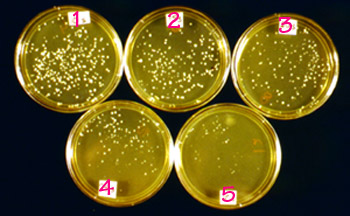
\includegraphics[width=1\textwidth]{images_20170912_yeast.jpeg}
     	\end{center}
	\end{column}
\end{columns}
\end{frame}

%------------------------------------------------
\begin{frame}
\frametitle{A Parable}
\begin{columns}
	\begin{column}{0.5\textwidth}
		\begin{itemize}
			\item<+-> Each plate contains .8\% lactose agar
			\item<+-> At the end of a week the measure the gene expression of each
			\item<+-> What is wrong with this ``experiment''?
		\end{itemize}
		\end{column}
	\begin{column}{0.5\textwidth}
		\begin{center}
     		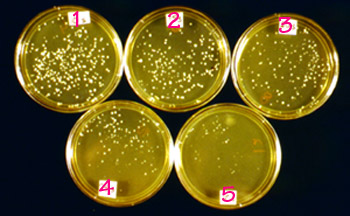
\includegraphics[width=1\textwidth]{images_20170912_yeast.jpeg}
     	\end{center}
	\end{column}
\end{columns}
\end{frame}

%------------------------------------------------
\begin{frame}
\frametitle{Dotstorming Check-In}
\begin{itemize}
	\item Did I cover the top questions?
	\item \href{https://dotstorming.com/b/59b6a35f3b45421106effc50}{Dotstorming Board}
\end{itemize}
\end{frame}

%------------------------------------------------
\begin{frame}
\frametitle{Learning to Code (and other skills)}
\end{frame}

%------------------------------------------------
\begin{frame}
\frametitle{Learning to Code (and other skills)}
\centerline{
\includegraphics[width=0.8\textwidth]{images_20170912_skills.png}}
\end{frame}

%------------------------------------------------
\section{Project Groups}
%------------------------------------------------

%------------------------------------------------
%%UNCOMMENT
\begin{frame}
\frametitle{Meet your Group!}
	\begin{itemize}
	\item<1-> Jennifer, Nayib, Chris
	\item<2-> Austin, Alan, Raymond
	\item<3-> Othmane, Kevin, Alvin
	\item<4-> Helena, Jake, Rahul
	\item<5-> Hank, Sisi, Joy
	\end{itemize}
\end{frame}

%------------------------------------------------
\begin{frame}
	\begin{itemize}
		\item<+-> {\Large Today's Tasks:}
		\item<+-> Meet with your group
		\item<+-> Discuss common interests
		\item<+-> Exchange and ideas or datasets you had hoped to use
		\item<+-> Leave with a plan to find data by next Tuesday
	\end{itemize}
\end{frame}


%------------------------------------------------
\begin{frame}
\Huge{\centerline{The End}}
\end{frame}

%----------------------------------------------------------------------------------------

\end{document} 